\documentclass[sn-mathphys-num]{sn-jnl}
\usepackage{graphicx}%
\usepackage{multirow}%
\usepackage{amsmath,amssymb,amsfonts}%
\usepackage{amsthm}%
\usepackage[mathscr]{mathalpha}%
\usepackage[title]{appendix}%
\usepackage{xcolor}%
\usepackage{textcomp}%
\usepackage{manyfoot}%
\usepackage{booktabs}%
\usepackage{algorithm}%
\usepackage{algorithmicx}%
\usepackage{algpseudocode}%
\usepackage{listings}%
\usepackage{lmodern}


\raggedbottom
\begin{document}
\title[Article Title]{Application of LSTM Neural Networks and Complex Network Analysis for Earthquake Forecasting in Colombia}

%%=============================================================%%
%% GivenName	-> \fnm{Joergen W.}
%% Particle	-> \spfx{van der} -> surname prefix
%% FamilyName	-> \sur{Ploeg}
%% Suffix	-> \sfx{IV}
%% \author*[1,2]{\fnm{Joergen W.} \spfx{van der} \sur{Ploeg} 
%%  \sfx{IV}}\email{iauthor@gmail.com}
%%=============================================================%%

\author*[1]{\fnm{Santiago} \sur{Giraldo}}\email{giraldo.santiago@correounivalle.edu.co.com}

\author[2]{\fnm{Daniel} \sur{León}}\email{daniel.leon@correounivalle.edu.co}
\equalcont{These authors contributed equally to this work.}

\author[3]{\fnm{Victor} \sur{Bucheli}}\email{victor.bucheli@correounivalle.edu.co}
\equalcont{These authors contributed equally to this work.}

\affil*[1,2,3]{\orgdiv{Escuela de Ingeniería de Sistemas}, \orgname{Universidad del Valle}, \orgaddress{\street{13th st.}, \city{Cali}, \postcode{760033}, \state{Valle del Cauca}, \country{Colombia}}}


\abstract{
    Earthquakes are unexpected and high risk events that may cause human casualties and damage to infrastructures.
    Over the last years, there's been an increasing amount of earthquake forecasting research in machine learning and neural 
    networks with astonishing results. This work approaches the earthquake forecasting problem with an application of 
    Long Short-Term Memory (LSTM) Neural Networks to historical seismic events in Colombia's pacific shore retrieved from 
    the United States Geological Survey service. We analyzed the seismic catalog over the time, included complex networks 
    features for each set, and trained multiple LSTM neural networks with hyper-parameter tuning. 
    We also used features like latitude, longitude, magnitude, days elapsed between events and complex networks properties. 
    We found models with \( R^2 \) score greater than 98\% when targeting multiple features at once, and greater than 99\% when 
    targeting one feature.
}

\keywords{Earthquake Forecasting, LSTM Neural Networks, Machine Learning, Complex Networks}
\maketitle
\section{Introduction}\label{introduction}

Earthquakes are classified a high risk event due to their unexpected nature and the limited time available to take preventive actions. Furthermore, the earthquakes may cause the human casualties and infrastructure damage. Over the past few years, numerous papers have explored the use of machine learning algorithms and neural networks for earthquake forecasting \cite{banna_application_2020, florido_earthquake_2016, mignan_neural_2020, jiao_artificial_2020, galkina_machine_nodate, kong_machine_2019}. The growing interest in the use of machine learning has been documented, as well as the use of artificial intelligence to forecast seismic events, indicating future work and various challenges to be addressed.

One approach involves the application of deep neural networks to learn from data directly to identify complex patterns, though, the forecasting of features such as magnitude, is limited by the lack of events that exceed certain threshold [REFERENCIAS]. The most interesting approach, uses a set of different characteristics and regions as input to the neural network in a moving window of time \cite{wang_earthquake_2020}. 

Some of the documented features in literature are magnitude, frequency of events \cite{han_medium-_1997,de_falco_seismicity_2000,bodri_neural-network_2001,wang_support_2006,sri_lakshmi_model_2009}, occurrence of aftershocks \cite{lin_forecast_2002}, probability of detection and rate of false alarms \cite{panakkat_neural_2007} , geomagnetic field variation, soil temperature and relative humidity \cite{suratgar_magnitude_2008}, seismic indicators \cite{panakkat_recurrent_2009}, location \cite{veri_earthquake_2012}, Gutenberg-Richter b-value \cite{morales-esteban_earthquake_2013,reyes_neural_2013,asenciocortes_earthquake_2018}, gravity, georesistivity and water level \cite{cai_anomaly_2019}, elapsed days, mean magnitude, mean time between characteristic events, coefficient of variation of the mean time \cite{banna_attention-based_2021}, and electronic signals captured on seismographs \cite{bose_preseis_2008,lakkos_neural_1994,rovithakis_neural_2000,ifantis_support_2003,radeva_real-time_2005,bernardo-torres_one-step_2009}.

Artificial intelligence and machine learning algorithms are powerful tools to address a wide set of classification and forecasting problems. They have the potential to learn from hidden patterns within the provided data \cite{kong_machine_2019}. As seen in \cite{kong_machine_2019, bose_preseis_2008} their application in earthquake forecasting is useful for risk assessment and early prevention. 

In \cite{jiao_artificial_2020} is stated that studies in seismology are carried out for the following objectives: actions to reduce long-term disasters generated by earthquakes, preparation and adjustment to disasters, disaster response strategies and post-disaster recovery planning. To Satriano et al \cite{satriano_earthquake_2011}, information systems focused on the early warning of seismological events must quickly and reliably provide information on different parameters such as location, time, and size in order to improve the emergency response, and Espinosa et al \cite{espinosa-aranda_evolution_2009} mention that the Mexican SAS (seismic alert system), an early warning system, implemented in Mexico has allowed seismic waves to be detected up to 60 seconds in advance, a time frame that allows security procedures to be executed to protect equipment susceptible to damage such as power plants, computer systems. and communication networks.

Additionally, there has been an increasing interest to represent data through graphs, as complex relationships can be modeled using nodes and edges \cite{chami_machine_2021}, we can model earthquakes as a complex network representing the location as nodes and the sequence as edges \cite{leon_modeling_2018}. Learning from these structures has been successfully applied in particle interaction, recommendation systems, molecular properties, natural language processing, and others \cite{grattarola_graph_2020}.

As stated by León et al \cite{leon_modeling_2018}
seismological events as complex networks allows to study the seismicity in a region and unravel the relationship among these events. The earthquake networks are based on the temporal sequence of events and their specific location, different network features like path length, degree distribution, and clustering lead to define high relation between events, hubs and small-worldness network properties. Thus, integrating the analysis of complex networks to structure the relationship between seismic events seems to be helpful to improve forecast results.

In this document we processed Colombian earthquake data and trained various neural network models with LSTM layers. We found a LSTM-NN with X layers and activation functions, this model displays a R2 MSE MAE scores of ZZZ/WWW, proposed models compares training with earthquake features alone, and the addition of complex network features. Finding out the addition of complex network features IMPROVE/WORSEN the forecast, results are promising and offer XXXXX at seismic events in the region


\section{Methods}\label{methods}

In this section, we take a look at the training and test data, and the steps to generate the earthquake features used later for training.

The earthquake events used in this study were obtained from the U.S. Geological Survey (USGS) for the Colombian region, with latitudes ranging from -0.132° to 9.796° and longitudes from -80.343° to -72.466°. The events are plotted by magnitude and depth in \textbf{Figure \ref{fig1}}. The retrieved dataset contained 5462 events since 1975, which was reduced to 5025 events after processing. The data cleaning process involved removing empty values, converting string values to numerical values for certain features, and filtering out events that were not validated by multiple sources, had missing data points, or had zero values. The selected events were of the mb type, representing the body wave magnitude, and included the depth of the event.

\begin{figure}[H]
    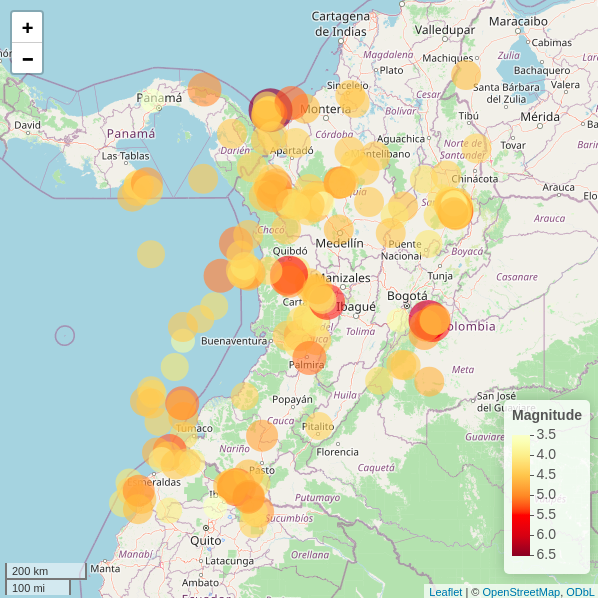
\includegraphics[width=0.49\textwidth]{img/mag01.png}
    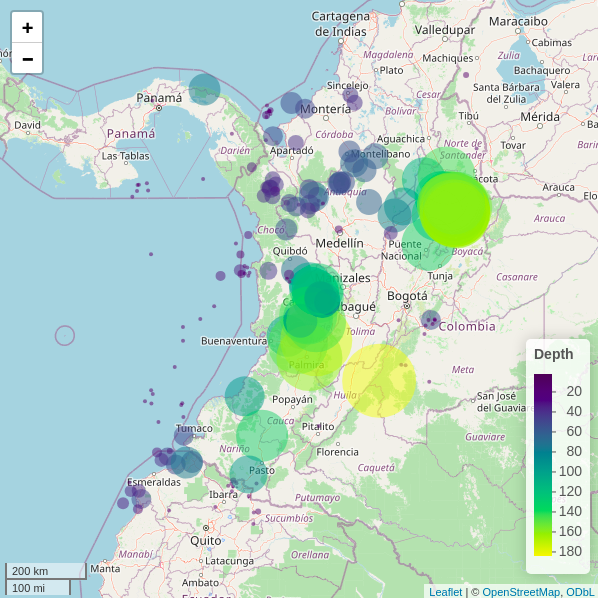
\includegraphics[width=0.49\textwidth]{img/depth01.png}
    \caption{Earthquake events by Magnitude (left) and Depth (right)}\label{fig1}
\end{figure}


\begin{table}[h]
    \caption{Caption text}\label{tab1}%
    \begin{tabular}{@{}llllllll@{}}
        \toprule
        Feature   & Min    & Max    & Median & Mean   & SD    & Variance & Range  \\
        \midrule
        Latitude  & -0.13  & 9.79   & 6.73   & 5.73   & 2.08  & 4.31     & 9.92   \\
        Longitude & -80.34 & -72.47 & -75.68 & -75.55 & 2.49  & 6.20     & 7.88   \\
        Depth     & 0.00   & 436.50 & 68.10  & 89.68  & 65.50 & 4290.78  & 436.50 \\
        Magnitude & 0.00   & 7.80   & 4.40   & 4.19   & 0.99  & 0.97     & 7.80   \\
        \botrule
    \end{tabular}
    \footnotetext{Source: This is an example of table footnote. This is an example of table footnote.}
    \footnotetext[1]{Example for a first table footnote. This is an example of table footnote.}
    \footnotetext[2]{Example for a second table footnote. This is an example of table footnote.}
\end{table}


\subsection{Earthquake Networks}\label{earthquake_networks}
Following the methodology proposed by Leon et al. \cite{leon_modeling_2018}, constructing an Earthquake Complex Network involves dividing the selected geographical area into a grid of cells, each representing a specific distance in kilometers. Sequential earthquake events are then used to establish connections between these cells, forming the network.

\begin{figure}[H]
    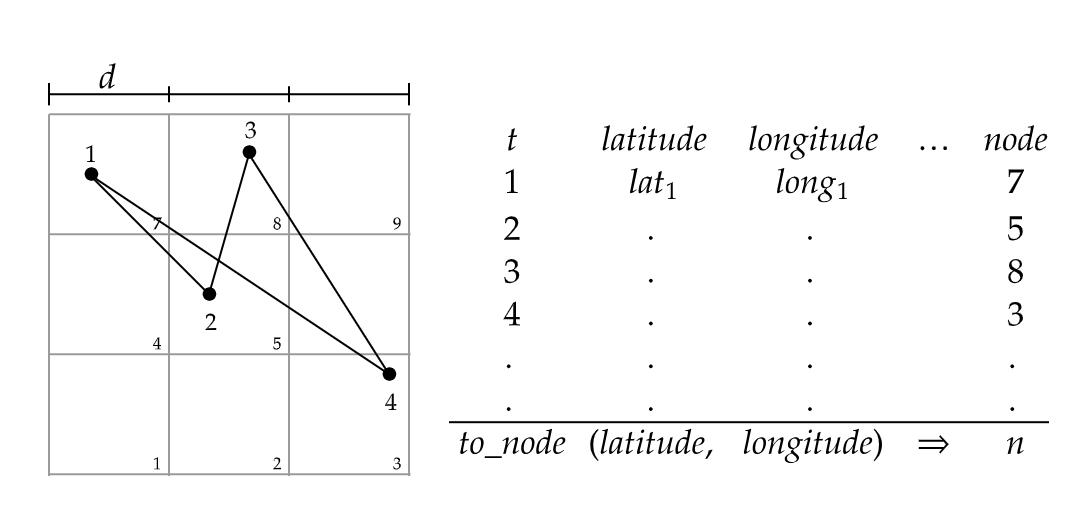
\includegraphics[width=1\textwidth]{img/diagram-20250202.png}
    \caption{Illustration of the creation of an earthquake network. \textbf{a)} A geographical region is divided into cells of equal size, with earthquakes represented as black dots. Each number identifies an event by its order in the time sequence, and a cell is selected if an earthquake occurs within it. \textbf{b)} The selected cells are used as nodes in the network, connected according to the time sequence. The brackets near each link indicate the events that caused the connection.\label{fig2}}
\end{figure}
\unskip

\subsection{Dataset}\label{dataset}

After we had the processed and cleansed the data,  we proceeded to tag each one of the events with their corresponding node. After this, we normalized all the features using scikit-learn StandardScaler.

Following the methodology proposed by Lin et al. \cite{lai_modeling_2018}, multivariate time-series forecasting involves using a rolling window approach. In this context, the input to the model is a sequence of values \( \{y_1, y_2, \ldots, y_l\} \), and the output is the value \( y_{l+l} \), where \( l \) represents the lookback number of events. We applied this approach to the earthquake data, using the features within each window as inputs to the neural network and the selected features of the subsequent event as the target.

The sequences were explored according to the lookback parameter during, we generated different matrices of size \( (S, L) \) resulting in a dataset of size \( (N, S, L)\). The following figure shows the structure of the dataset for the LSTM network.

\begin{figure}[H]
    \centering
    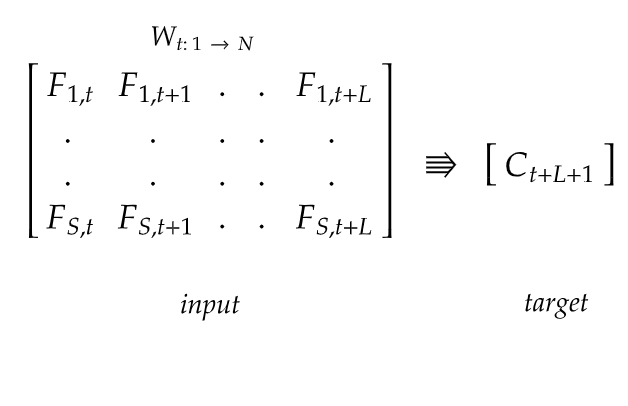
\includegraphics[width=0.6\textwidth]{img/dataset-diagram.png}
    \caption{Dataset for the LSTM neural network.\label{fig2}}
\end{figure}
\unskip


To calculate the complex network properties, we took each moving window and built the respective graph, taking cell distance values of 10, 50, and 100 kilometers, per each event sequence of 50 and 100 events.
The networks features we included in the moving windows were degree centrality, clustering, betweenness centrality, closeness centrality, and page rank. 

% Topical subheadings are allowed. Authors must ensure that their Methods section includes adequate experimental and characterization data necessary for others in the field to reproduce their work. Authors are encouraged to include RIIDs where appropriate. 

% \begin{enumerate}[1.]
% \item Approval: a statement which confirms that all experimental protocols were approved by a named institutional and/or licensing committee. Please identify the approving body in the methods section

% \item Accordance: a statement explicitly saying that the methods were carried out in accordance with the relevant guidelines and regulations

% \item Informed consent (for experiments involving humans or human tissue samples): include a statement confirming that informed consent was obtained from all participants and/or their legal guardian/s
% \end{enumerate}


\section{Results}\label{sec2}

Sample body text. Sample body text. Sample body text. Sample body text. Sample body text. Sample body text. Sample body text. Sample body text.

\section{Discussion}\label{sec12}

Discussions should be brief and focused. In some disciplines use of Discussion or `Conclusion' is interchangeable. It is not mandatory to use both. Some journals prefer a section `Results and Discussion' followed by a section `Conclusion'. Please refer to Journal-level guidance for any specific requirements. 

\section{Conclusion}\label{sec13}

Conclusions may be used to restate your hypothesis or research question, restate your major findings, explain the relevance and the added value of your work, highlight any limitations of your study, describe future directions for research and recommendations. 

In some disciplines use of Discussion or 'Conclusion' is interchangeable. It is not mandatory to use both. Please refer to Journal-level guidance for any specific requirements. 

\backmatter

\bmhead{Supplementary information}

If your article has accompanying supplementary file/s please state so here. 

Authors reporting data from electrophoretic gels and blots should supply the full unprocessed scans for key as part of their Supplementary information. This may be requested by the editorial team/s if it is missing.

Please refer to Journal-level guidance for any specific requirements.

\bmhead{Acknowledgements}

Acknowledgements are not compulsory. Where included they should be brief. Grant or contribution numbers may be acknowledged.

Please refer to Journal-level guidance for any specific requirements.

\section*{Declarations}

Some journals require declarations to be submitted in a standardised format. Please check the Instructions for Authors of the journal to which you are submitting to see if you need to complete this section. If yes, your manuscript must contain the following sections under the heading `Declarations':

\begin{itemize}
    \item Funding
    \item Conflict of interest/Competing interests (check journal-specific guidelines for which heading to use)
    \item Ethics approval and consent to participate
    \item Consent for publication
    \item Data availability
    \item Materials availability
    \item Code availability
    \item Author contribution
\end{itemize}

\noindent
If any of the sections are not relevant to your manuscript, please include the heading and write `Not applicable' for that section. 

%%===================================================%%
%% For presentation purpose, we have included        %%
%% \bigskip command. Please ignore this.             %%
%%===================================================%%
\bigskip
\begin{flushleft}%
    Editorial Policies for:
    
    \bigskip\noindent
    Springer journals and proceedings: \url{https://www.springer.com/gp/editorial-policies}
    
    \bigskip\noindent
    Nature Portfolio journals: \url{https://www.nature.com/nature-research/editorial-policies}
    
    \bigskip\noindent
    \textit{Scientific Reports}: \url{https://www.nature.com/srep/journal-policies/editorial-policies}
    
    \bigskip\noindent
    BMC journals: \url{https://www.biomedcentral.com/getpublished/editorial-policies}
\end{flushleft}

\begin{appendices}

    \section{Section title of first appendix}\label{secA1}
    
    An appendix contains supplementary information that is not an essential part of the text itself but which may be helpful in providing a more comprehensive understanding of the research problem or it is information that is too cumbersome to be included in the body of the paper.
    
    %%=============================================%%
    %% For submissions to Nature Portfolio Journals %%
    %% please use the heading ``Extended Data''.   %%
    %%=============================================%%
    
    %%=============================================================%%
    %% Sample for another appendix section			       %%
    %%=============================================================%%
    
    %% \section{Example of another appendix section}\label{secA2}%
    %% Appendices may be used for helpful, supporting or essential material that would otherwise 
    %% clutter, break up or be distracting to the text. Appendices can consist of sections, figures, 
    %% tables and equations etc.
    
\end{appendices}

%%===========================================================================================%%
%% If you are submitting to one of the Nature Portfolio journals, using the eJP submission   %%
%% system, please include the references within the manuscript file itself. You may do this  %%
%% by copying the reference list from your .bbl file, paste it into the main manuscript .tex %%
%% file, and delete the associated \verb+\bibliography+ commands.                            %%
%%===========================================================================================%%

\bibliographystyle{plain}
\bibliography{article}% common bib file
%% if required, the content of .bbl file can be included here once bbl is generated
%%\input sn-article.bbl


\end{document}
